\documentclass[12pt,a4paper]{report}
\usepackage[utf8]{inputenc}
\usepackage[T5]{fontenc}
\usepackage[vietnamese]{babel}
\usepackage{geometry}
\geometry{a4paper, left=3cm, right=2cm, top=2.5cm, bottom=2.5cm, headheight=15pt}
\usepackage{graphicx}
\usepackage{hyperref}
\usepackage{tabularx}
\usepackage{longtable}
\usepackage{booktabs}
\usepackage{array}
\usepackage{enumitem}
\usepackage{float}
\usepackage{titlesec}
\titleformat{\chapter}[hang]{\normalfont\LARGE\bfseries}{\thechapter.}{1em}{}
\titlespacing*{\chapter}{0pt}{30pt}{20pt}
\usepackage{fancyhdr}
\usepackage{indentfirst}
\usepackage{tikz}
\usetikzlibrary{calc}
% --- Page header/footer ---
\pagestyle{fancy}
\fancyhf{}
\fancyhead[L]{\small CO3001 -- Công nghệ Phần mềm -- HK261}
\fancyhead[R]{\small Nhóm BEE BRAVE}
\fancyfoot[C]{\thepage}
\renewcommand{\headrulewidth}{0.4pt}

\fancypagestyle{plain}{
  \fancyhf{}
  \fancyhead[L]{\small CO3001 -- Công nghệ Phần mềm -- HK261}
  \fancyhead[R]{\small Nhóm BEE BRAVE}
  \fancyfoot[C]{\thepage}
  \renewcommand{\headrulewidth}{0.4pt}
}

\hypersetup{
    colorlinks=true,
    linkcolor=blue,
    filecolor=magenta,
    urlcolor=blue,
    pdftitle={Smart E-Mobility Hub -- Báo cáo Phân tích Yêu cầu Phần mềm},
    pdfauthor={Nhóm BEE BRAVE -- L02},
}

\begin{document}

% ============================================================
%                       TRANG BÌA
% ============================================================
\begin{titlepage}
    \noindent
    \begin{tikzpicture}[remember picture, overlay]
        \draw[line width = 3pt] ($(current page.north west) + (1.5cm,-1.0cm)$) rectangle ($(current page.south east) + (-0.5cm,1.0cm)$);
        \draw[line width = 1pt] ($(current page.north west) + (1.65cm,-1.15cm)$) rectangle ($(current page.south east) + (-0.65cm,1.15cm)$);
    \end{tikzpicture}%
    \centering
    \textbf{\large ĐẠI HỌC QUỐC GIA THÀNH PHỐ HỒ CHÍ MINH}\\[0.3cm]
    \textbf{\Large TRƯỜNG ĐẠI HỌC BÁCH KHOA}\\[0.2cm]
    \textbf{\large KHOA KHOA HỌC VÀ KỸ THUẬT MÁY TÍNH}\\[0.5cm]
    
    
\includegraphics[width=8cm]{mau.png}\\[0.5cm]

    \rule{\textwidth}{0.5pt}\\[1cm]

    {\fontsize{22}{26}\selectfont\textbf{BÁO CÁO PHÂN TÍCH\\YÊU CẦU PHẦN MỀM}}\\[0.4cm]
    {\Large\textbf{SUBMISSION \#1}}\\[0.8cm]

    {\large MÔN HỌC: \textbf{CÔNG NGHỆ PHẦN MỀM (CO3001)} --- HK261}\\[0.4cm]
    {\large ĐỀ TÀI:}\\[0.2cm]
    {\Large\textbf{SMART E-MOBILITY HUB}}\\[0.2cm]
    {\large Hệ thống Điều phối Phương tiện Điện\\trong Khu đô thị ĐHQG-HCM}\\[1cm]

    \rule{\textwidth}{0.5pt}\\[0.8cm]

    \begin{flushleft}
        \hspace{1cm}\textbf{Giảng viên hướng dẫn:} TS. Trần Thị Ngọc Trâm\\[0.3cm]
        \hspace{1cm}\textbf{Lớp học phần:} L02\\[0.3cm]
        \hspace{1cm}\textbf{Nhóm báo cáo:} BEE BRAVE (7 thành viên)\\[0.2cm]
    \end{flushleft}
    \vfill
    Thành phố Hồ Chí Minh, Tháng 09/2026
\end{titlepage}
\setcounter{page}{1}
\newpage

% ============================================================
%                       DANH SÁCH NHÓM
% ============================================================

    \vspace*{\fill}
    \begin{center}
        \renewcommand{\arraystretch}{1.5}
        \begin{tabularx}{\textwidth}{|c|X|c|X|c|c|}
            \hline
            \textbf{STT} & \textbf{Họ và Tên} & \textbf{MSSV} & \textbf{Phân hệ phụ trách} & \textbf{Vai trò} & \textbf{Đóng góp} \\
            \hline
            1 & Nguyễn Thành Đạt & 2410709 & SS1: Đặt \& Quản lý Xe dùng chung & Leader/PM & 100\% \\
            \hline
            2 & Nguyễn Anh Tài & 2413035 & SS2: Đăng ký Sạc \& Đỗ xe cá nhân & Dev/Analyst & 100\% \\
            \hline
            3 & Phạm Tiến Đạt & 2410724 & SS3: Giám sát Mạng lưới Hub & Dev/Analyst & 100\% \\
            \hline
            4 & Đặng Hoàng Quý Nhân & 2412401 & SS4: Điều phối \& Xử lý Sự cố & Dev/Analyst & 100\% \\
            \hline
            5 & Dương Đăng Khoa & 2411589 & SS5: Lập lịch Sạc Thông minh & Dev/Analyst & 100\% \\
            \hline
            6 & Hoàng Văn Tấn & 2213074 & SS6: Mô phỏng What-if Nhu cầu & Dev/Analyst & 100\% \\
            \hline
            7 & Nguyễn Trung Nguyên & 2011710 & SS7: Mô phỏng What-if Hạ tầng & Dev/Analyst & 100\% \\
            \hline
        \end{tabularx}
    \end{center}
    \vspace*{\fill}
\newpage

% ============================================================
%                       MỤC LỤC
% ============================================================
\tableofcontents
\newpage

% ============================================================
%                    LỜI NÓI ĐẦU
% ============================================================
\chapter*{Lời nói đầu}
\addcontentsline{toc}{chapter}{Lời nói đầu}

Trong bối cảnh thời đại số hóa và sự phát triển mạnh mẽ của các mô hình đô thị thông minh, việc vận dụng các kiến thức từ môn Công nghệ phần mềm vào giải quyết các bài toán giao thông thực tiễn ngày càng đóng vai trò thực tiễn. 
Đối với sinh viên khối ngành kỹ thuật tại Trường Đại học Bách Khoa - ĐHQG-HCM, môn học Công nghệ Phần mềm (CO3001) không chỉ cung cấp nền tảng lý thuyết vững chắc về quy trình phân tích yêu cầu (SRS), thiết kế kiến trúc 
và quản lý cấu hình, mà còn trang bị phương pháp tư duy khoa học để tiếp cận và mô hình hóa các hệ thống phần mềm phân tán phức tạp.


Nhằm hiện thực hóa những kiến thức đã học trên giảng đường, Nhóm BEE BRAVE tiến hành đi sâu nghiên cứu đề tài: "\textit{Smart E-Mobility Hub - Hệ thống Điều phối Phương tiện Điện trong Khu đô thị ĐHQG-HCM}". 
Mục tiêu cốt lõi của đề tài là xây dựng một nền tảng quản lý tập trung nhằm tối ưu hóa mạng lưới xe điện dùng chung, xe cá nhân, bãi đỗ và trạm sạc, phục vụ nhu cầu di chuyển, kết nối ga Metro Tuyến số 1 với các cơ sở đào tạo và ký túc xá. 
Trong khuôn khổ báo cáo Submission \#1, nhóm tập trung đặc tả toàn diện 17 Use-cases thuộc 7 phân hệ nghiệp vụ, thiết kế Sơ đồ Use-case tổng thể hệ thống, liệt kê được các yêu cầu chức năng (functional requirements) và phi chức năng (non-functional requirements), đồng thời thiết lập quy trình kiểm định chất lượng (QA Audit) và quản lý cấu hình mã nguồn nghiêm ngặt.


Bài tập lớn lần này thực sự là một cơ hội quý báu để 7 thành viên trong nhóm rèn luyện tư duy logic, nâng cao kỹ năng phân tích nghiệp vụ và trải nghiệm quy trình phát triển phần mềm nhóm chuyên nghiệp trên GitHub. Dù đã nỗ lực tìm hiểu và hoàn thiện bài làm, song với những giới 
hạn nhất định về mặt kinh nghiệm thực tiễn, báo cáo chắc chắn vẫn không tránh khỏi những thiếu sót. Nhóm chúng em rất mong nhận được những nhận xét, đánh giá và lời góp ý tận tình từ Cô Trần Thị Ngọc Trâm để nhóm có thể khắc phục hạn chế và tiếp tục hoàn thiện sản phẩm trong các giai đoạn tiếp theo. Nhóm chúng em xin chân thành cảm ơn Cô!

% ============================================================
%   CHƯƠNG 1: ĐẶC TẢ CHI TIẾT DỰ ÁN
% ============================================================
\chapter{Đặc tả Chi tiết Dự án (Project Details Specification)}

\section{Bối cảnh dự án (Project Context)}
Khu đô thị ĐHQG-HCM bao gồm nhiều trường đại học thành viên (Bách Khoa, Khoa học Tự nhiên, Công nghệ Thông tin, ...), ký túc xá sinh viên (Khu A, Khu B), khu dịch vụ thương mại (Canteen, Thư viện Trung tâm), và ga Metro Tuyến số 1 --- điểm trung chuyển chính kết nối với hệ thống giao thông công cộng thành phố. Khoảng cách giữa ga Metro và các cơ sở đào tạo có thể lên tới 2--4 km, gây ra nhu cầu lớn về phương tiện di chuyển ``chặng cuối'' (Last-Mile).

Hệ thống Smart E-Mobility Hub được đề xuất nhằm giải quyết bài toán này bằng cách cung cấp mạng lưới các trạm xe điện dùng chung kết hợp dịch vụ đỗ xe và sạc điện cho xe cá nhân.

\section{Mục tiêu dự án (Objectives)}

Cung cấp nền tảng quản lý tập trung cho mạng lưới các Hub xe điện phân tán.

Tự động hóa quy trình đặt chỗ, nhận xe, trả xe và quyết toán chi phí qua ví điện tử nội bộ.

Tối ưu hóa lập lịch sạc dựa trên thuật toán chấm điểm ưu tiên (SoC, thời gian chờ, giá điện theo giờ).

Cân bằng tải phương tiện giữa các Hub thông qua lệnh điều phối tự động.

Hỗ trợ ra quyết định thông qua mô phỏng What-if (Metro Surge \& Power Outage).

\section{Phạm vi và Ranh giới (Scope \& Boundaries)}

\subsection{Trong phạm vi (In-Scope)}

\textbf{Quản lý trạng thái (State Management):} Theo dõi và chuyển đổi trạng thái xe, cổng sạc, slot đỗ (AVAILABLE $\rightarrow$ RESERVED $\rightarrow$ IN\_USE $\rightarrow$ COMPLETED / CANCELLED).

\textbf{Phân bổ tài nguyên (Resource Allocation):} Cấp phát slot đỗ xe, cổng sạc, phương tiện dựa trên khả dụng thời gian thực.

\textbf{Đặt chỗ \& Vòng đời dịch vụ:} Đặt giữ chỗ xe 15 phút, đặt cọc ví điện tử, nhận/trả xe, hủy \& hoàn cọc, e-invoice.

\textbf{Lập lịch sạc thông minh:} Thuật toán chấm điểm ưu tiên sạc (SoC, thời gian chờ, mức khẩn cấp, giá điện peak/off-peak), hàng đợi sạc, cảnh báo overstay.

\textbf{Điều phối phương tiện:} Lệnh điều chuyển xe giữa các Hub để cân bằng tải, xử lý sự cố.

\textbf{Mô phỏng What-if:} Mô phỏng Metro Surge, lỗi cổng sạc, mất điện trạm, đánh giá tác động và đề xuất điều hướng.

\textbf{Giám sát \& Cảnh báo:} Dashboard KPI thời gian thực, cảnh báo phân cấp ngưỡng chiếm dụng (70\% / 85\% / 100\%).

\subsection{Ngoài phạm vi (Out-of-Scope)}

Phần cứng IoT vật lý --- dự án sử dụng dữ liệu cảm biến mô phỏng (mock/simulated data).

Giao diện bản đồ 3D / GIS --- trọng tâm đặt vào logic nghiệp vụ.

Tích hợp cổng thanh toán ngân hàng thật --- sử dụng ví điện tử mô phỏng (in-memory wallet).

Xác thực VNU-SSO thực tế --- sử dụng mock authentication.

Ứng dụng di động native (iOS/Android) --- hệ thống hướng tiếp cận linh hoạt, tạo nền tảng Web có thể deploy locally hoặc sử dụng Docker tuỳ thuộc vào định hướng phát triển ở các giai đoạn sau (prototype hiện tại chạy trên nền Streamlit).

\section{Phân tích Bên liên quan (Stakeholders)}

\renewcommand{\arraystretch}{1.5}
\begin{longtable}{|>{\bfseries\raggedright}p{3cm}|>{\raggedright\arraybackslash}p{3.5cm}|>{\raggedright\arraybackslash}p{6cm}|>{\raggedright\arraybackslash}p{2.5cm}|}
    \hline
    \textbf{Nhóm} & \textbf{Vai trò} & \textbf{Kỳ vọng \& Mô tả} & \textbf{Subsystem} \\
    \hline
    \endfirsthead
    \hline
    \textbf{Nhóm} & \textbf{Vai trò} & \textbf{Kỳ vọng \& Mô tả} & \textbf{Subsystem} \\
    \hline
    \endhead

    Khối Sinh viên (End-Users) & Sinh viên thuê xe chung & Sử dụng bãi đỗ chung, đặt xe giữ chỗ, thanh toán qua ví nội bộ, xem hóa đơn. & SS1 \\
    \hline
    & Sinh viên gửi/sạc xe cá nhân & Đăng ký thông tin xe, đặt trước vị trí, tính phí sạc/đỗ và thanh toán. & SS2, SS5 \\
    \hline
    Nhân viên Vận hành Hub & Nhân viên giám sát trung tâm & Theo dõi trạng thái Hub, nhận cảnh báo quá tải, đối soát doanh thu. & SS3, SS1, SS2 \\
    \hline
    Kỹ thuật viên & Kỹ thuật viên hiện trường & Điều phối phương tiện, xử lý sự cố tại bãi đỗ và trạm sạc. & SS4 \\
    \hline
    Hệ thống Ngoại vi (External) & Tuyến Metro số 1 & Cung cấp dữ liệu về lưu lượng hành khách, tần suất các chuyến tàu đến. & SS6 \\
    \hline
    & Mạng lưới IoT & Thu thập dữ liệu thời gian thực (trạng thái cổng sạc, kWh, cảm biến). & SS3, SS4, SS5 \\
    \hline
    & Ví điện tử nội bộ & Xử lý giao dịch nạp tiền, trừ phí, hoàn cọc tự động và kết xuất biên nhận. & SS1, SS2, SS5 \\
    \hline
\end{longtable}

% ============================================================
%   CHƯƠNG 2: YÊU CẦU CHỨC NĂNG
% ============================================================
{\let\clearpage\relax
\chapter{Yêu cầu Chức năng (Functional Requirements)}}

\section{Danh sách User Stories}

\subsection{SS1 -- Quản lý \& Đặt xe cho Sinh viên}
\begin{enumerate}[nosep,label=\textbf{US-\arabic*:}]
    \item \textit{Là một sinh viên,} tôi muốn \textbf{đặt một chỗ đỗ xe chung} để có chỗ đỗ bảo mật khi tới campus.
    \item \textit{Là một sinh viên,} tôi muốn \textbf{tra cứu danh sách xe điện khả dụng kèm mức pin (SoC \%) và đơn giá thuê minh bạch} (VNĐ/phút hoặc miễn phí 30 phút đầu cho SV ĐHQG-HCM) để chủ động lựa chọn phương tiện.
    \item \textit{Là một sinh viên,} tôi muốn \textbf{thanh toán tiền cọc tạm tính qua ví điện tử nội bộ và khóa giữ chỗ xe trong 15 phút} để đảm bảo xe không bị người khác lấy.
\end{enumerate}
\begin{enumerate}[nosep,label=\textbf{US-\arabic*b:}]
    \setcounter{enumi}{2}
    \item \textit{Là một sinh viên đã đặt giữ chỗ xe,} tôi muốn \textbf{quét mã QR/PIN tại Hub để Nhận xe (Pick-up)} để mở khóa phương tiện và bắt đầu tính thời gian di chuyển.
\end{enumerate}
\begin{enumerate}[nosep,label=\textbf{US-0\arabic*:},start=4]
    \item \textit{Là một sinh viên,} tôi muốn \textbf{áp dụng mã giảm giá / voucher sinh viên} khi đặt xe để được hưởng ưu đãi.
    \item \textit{Là một sinh viên,} tôi muốn \textbf{hủy đặt chỗ và được hoàn trả 100\% tiền cọc} nếu thay đổi kế hoạch trong thời hạn 15 phút.
\end{enumerate}
\begin{enumerate}[nosep,label=\textbf{US-\arabic*b:}]
    \setcounter{enumi}{4}
    \item \textit{Là một sinh viên đang sử dụng xe,} tôi muốn \textbf{Trả xe (Return Vehicle) tại Hub điểm đến} để kết thúc chuyến đi và tự động quyết toán chi phí thuê xe vào ví.
\end{enumerate}
\begin{enumerate}[nosep,label=\textbf{US-0\arabic*:},start=6]
    \item \textit{Là một sinh viên,} tôi muốn \textbf{xem hóa đơn điện tử chi tiết sau chuyến đi} để quản lý chi tiêu minh bạch.
    \item \textit{Là một quản trị viên,} tôi muốn \textbf{xem danh sách đặt chỗ hiện tại và doanh thu dịch vụ xe chung} để quản lý hiệu quả vận hành.
\end{enumerate}

\subsection{SS2 -- Đăng ký dịch vụ Xe cá nhân}
\begin{enumerate}[nosep,label=\textbf{US-\arabic*:},start=8]
    \item \textit{Là một sinh viên,} tôi muốn \textbf{đăng ký xe EV cá nhân (biển số, loại xe, dung lượng pin)} để hệ thống xác thực quyền đỗ xe và cấp quyền sạc.
    \item \textit{Là một chủ xe cá nhân,} tôi muốn \textbf{tra cứu biểu phí đỗ xe theo giờ và đặt trước vị trí đỗ} để an tâm có chỗ gửi xe.
    \item \textit{Là một chủ xe cá nhân,} tôi muốn \textbf{đặt lịch sạc và được tự động tính phí dựa trên kWh kết hợp khung giờ cao điểm / thấp điểm} để tối ưu chi phí.
    \item \textit{Là một chủ xe cá nhân,} tôi muốn \textbf{thanh toán tích hợp cả phí gửi xe và phí sạc trên một hóa đơn điện tử qua ví nội bộ} để tiết kiệm thời gian.
\end{enumerate}
\begin{enumerate}[nosep,label=\textbf{US-\arabic*b:}]
    \setcounter{enumi}{10}
    \item \textit{Là một chủ xe đã đặt trước chỗ đỗ/sạc,} tôi muốn \textbf{quét mã QR/biển số Check-in/Check-out tại barie tự động} để đảm bảo xe đỗ đúng vị trí được cấp phép.
\end{enumerate}
\begin{enumerate}[nosep,label=\textbf{US-\arabic*:},start=12]
    \item \textit{Là một nhân viên vận hành,} tôi muốn \textbf{kiểm tra trạng thái sạc, biểu phí và xác nhận thanh toán} để quyết định thứ tự ưu tiên sạc.
\end{enumerate}

\subsection{SS3 -- Giám sát mạng lưới Hub}
\begin{enumerate}[nosep,label=\textbf{US-\arabic*:},start=13]
    \item \textit{Là một nhân viên giám sát,} tôi muốn \textbf{xem dashboard tổng quan} về số lượng xe, mức độ sử dụng, doanh thu tạm tính và cảnh báo quá tải.
\end{enumerate}
\begin{enumerate}[nosep,label=\textbf{US-\arabic*b:}]
    \setcounter{enumi}{12}
    \item \textit{Là một nhân viên giám sát,} tôi muốn \textbf{hệ thống tự động kích hoạt cảnh báo phân cấp} (Vàng $\ge 70\%$, Đỏ $\ge 85\%$, Khóa $100\%$) để kịp thời điều phối.
\end{enumerate}
\begin{enumerate}[nosep,label=\textbf{US-\arabic*:},start=14]
    \item \textit{Là một kỹ thuật viên,} tôi muốn \textbf{nhận thông báo IoT khi cảm biến phát hiện lỗi} để kịp thời xử lý.
\end{enumerate}

\subsection{SS4 -- Điều phối \& Xử lý sự cố}
\begin{enumerate}[nosep,label=\textbf{US-\arabic*:},start=15]
    \item \textit{Là một điều phối viên,} tôi muốn \textbf{chỉ định xe từ Hub A sang Hub B} để cân bằng tải.
    \item \textit{Là một kỹ thuật viên hiện trường,} tôi muốn \textbf{báo cáo sự cố (va chạm, hết pin, hỏng), tiếp nhận xử lý và ghi nhận thời gian khắc phục} để phương tiện sớm khả dụng.
    \item \textit{Là một quản trị viên,} tôi muốn \textbf{xem lịch sử sự cố} để phân tích nguyên nhân.
\end{enumerate}

\subsection{SS5 -- Lập lịch sạc thông minh}
\begin{enumerate}[nosep,label=\textbf{US-\arabic*:},start=18]
    \item \textit{Là một chuyên viên sạc,} tôi muốn \textbf{tự động xếp hàng sạc dựa trên mức ưu tiên} (pin, thời gian, mức độ khẩn cấp, giá điện theo giờ).
    \item \textit{Là một sinh viên,} tôi muốn \textbf{được thông báo khi xe đã sạc xong và nhận biên nhận chi phí điện năng đã nạp}.
\end{enumerate}
\begin{enumerate}[nosep,label=\textbf{US-\arabic*b:}]
    \setcounter{enumi}{18}
    \item \textit{Là một chuyên viên trạm sạc,} tôi muốn \textbf{hệ thống tự động cảnh báo xe sạc đầy và áp dụng phí chiếm dụng (Overstay Fee)} nếu sau 15 phút ân hạn xe chưa được rút sạc.
\end{enumerate}
\begin{enumerate}[nosep,label=\textbf{US-\arabic*:},start=20]
    \item \textit{Là một quản trị viên,} tôi muốn \textbf{đặt giới hạn năng lượng tối đa (Peak Power Capping)} để tránh quá tải lưới điện.
\end{enumerate}

\subsection{SS6 -- Mô phỏng nhu cầu SV (What-if Demand)}
\begin{enumerate}[nosep,label=\textbf{US-\arabic*:},start=21]
    \item \textit{Là một nhà phân tích,} tôi muốn \textbf{mô phỏng tăng/giảm nhu cầu sinh viên dựa trên dữ liệu lưu lượng Ga Metro (Metro Surge)} để dự đoán tải và biến động doanh thu.
    \item \textit{Là một nhà quản lý,} tôi muốn \textbf{xem biểu đồ dự báo nhu cầu và phân tích phụ tải hàng đợi 24h} để lên kế hoạch mở rộng Hub.
\end{enumerate}

\subsection{SS7 -- Mô phỏng sự cố hạ tầng (What-if Infrastructure Failure)}
\begin{enumerate}[nosep,label=\textbf{US-\arabic*:},start=23]
    \item \textit{Là một kỹ thuật viên,} tôi muốn \textbf{kích hoạt mô phỏng lỗi cổng sạc hoặc mất điện trạm sạc} để kiểm tra quy trình phục hồi.
    \item \textit{Là một điều phối viên,} tôi muốn \textbf{xem ảnh hưởng của lỗi hạ tầng lên luồng xe} và đưa ra quyết định điều hướng.
\end{enumerate}
\begin{enumerate}[nosep,label=\textbf{US-\arabic*b:}]
    \setcounter{enumi}{23}
    \item \textit{Là một sinh viên đang di chuyển đến Hub gặp sự cố,} tôi muốn \textbf{nhận thông báo cảnh báo tự động và đề xuất điều hướng sang Hub lân cận còn chỗ trống} để không bị gián đoạn hành trình.
\end{enumerate}

\section{Sơ đồ Use-Case Tổng thể (Use-Case Diagram)}

Sơ đồ Use-Case tổng thể của hệ thống Smart E-Mobility Hub được thiết kế theo chuẩn UML với các thành phần sau:
\begin{itemize}[nosep]
    \item \textbf{Ranh giới hệ thống (System Boundary):} ``Smart E-Mobility Hub System'' bao bọc toàn bộ 17 Use-Case.
    \item \textbf{3 nhóm Tác nhân người dùng (Actors):} Khối Sinh viên, Nhân viên Vận hành Hub, Kỹ thuật viên.
    \item \textbf{1 Tác nhân hệ thống ngoại vi:} Hệ thống ngoại vi (Tuyến Metro / IoT / Ví điện tử).
    \item \textbf{Quan hệ UML:} Sử dụng \texttt{<<include>>} cho các luồng phụ thuộc bắt buộc và \texttt{<<extend>>} cho các luồng mở rộng tùy chọn.
\end{itemize}

\begin{figure}[H]
    \centering
    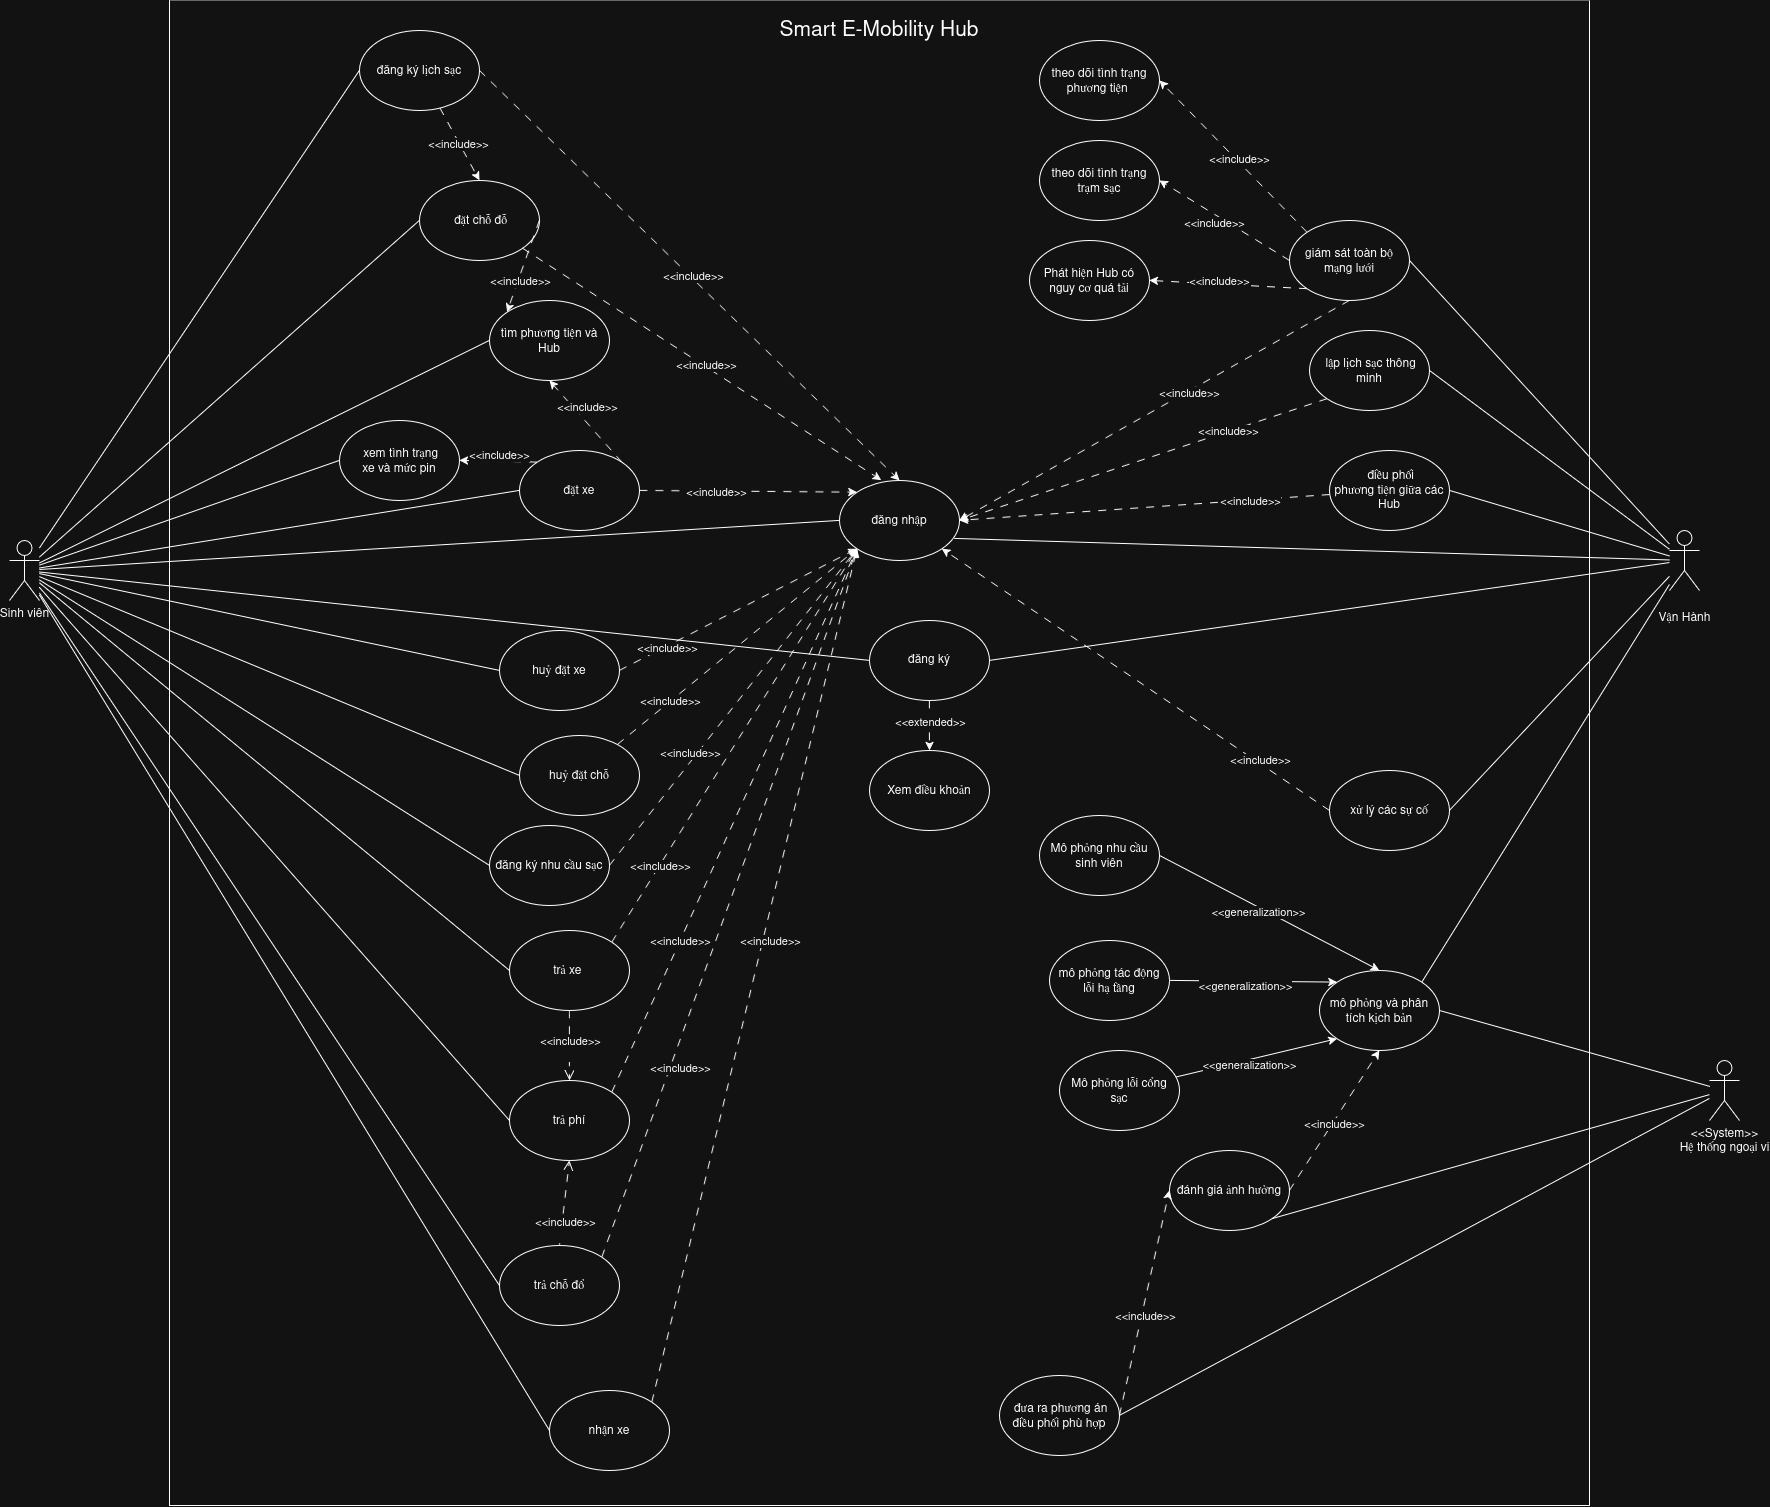
\includegraphics[width=\textwidth]{../diagrams/system/smartEhub.png}
    \caption{Sơ đồ Use-Case Tổng thể của Hệ thống Smart E-Mobility Hub}
    \label{fig:usecase-diagram}
\end{figure}

\section{Yêu cầu chức năng phi tương tác (Other Non-interactive FRs -- Bonus)}

Ngoài các nghiệp vụ tương tác trực tiếp với người dùng, hệ thống còn tích hợp các logic xử lý ngầm quan trọng:
\begin{itemize}[nosep]
    \item \textbf{FR-09 (Thuật toán lập lịch sạc tự động):} Hệ thống tự động chấm điểm và xếp hạng ưu tiên sạc dựa trên SoC hiện tại, thời gian chờ trong hàng đợi, mức độ khẩn cấp, và biểu giá điện theo giờ.
    \item \textbf{FR-10b (Giám sát chiếm dụng trụ sạc):} Daemon tự động phát hiện xe đã sạc đầy pin và áp dụng phí Overstay Fee (10,000 VNĐ/15 phút) nếu sau 15 phút ân hạn xe vẫn chưa được rút sạc.
    \item \textbf{FR-05c (Cảnh báo phân cấp quá tải):} Logic tự động kích hoạt cảnh báo theo 3 mức ngưỡng chiếm dụng Hub (Vàng $\ge 70\%$, Đỏ $\ge 85\%$, Khóa đặt chỗ khi $100\%$).
    \item \textbf{FR-12 (Sinh dữ liệu mô phỏng Metro Surge):} Background job tự động sinh ngẫu nhiên lưu lượng xe giả lập theo phân phối xác suất khi kích hoạt kịch bản Metro Surge.
    \item \textbf{FR-15c (Auto-rerouting):} Tự động quét tìm 02 Hub gần nhất còn chỗ trống và gửi thông báo gợi ý điều hướng kèm nút chuyển đặt chỗ 1-chạm.
\end{itemize}

\section{Đặc tả chi tiết Use-Case Scenarios (Individual Work)}

Tổng cộng \textbf{17/17 Use-cases} đã được mỗi thành viên đặc tả hoàn chỉnh bằng file Markdown và Word, tuân thủ theo yêu cầu từ đặc tả và ý kiến thống nhất qua các cuộc họp của nhóm sau khi phân tích đặc tả, stakeholder và user stories. Tài liệu chi tiết được lưu tại thư mục \texttt{docs/diagrams/Use-case detail-scenario/}.

\renewcommand{\arraystretch}{1.4}
\begin{longtable}{|c|l|l|l|c|}
    \hline
    \textbf{STT} & \textbf{Mã UC} & \textbf{Tên Use-Case} & \textbf{Thành viên} & \textbf{SS} \\
    \hline
    \endfirsthead
    \hline
    \textbf{STT} & \textbf{Mã UC} & \textbf{Tên Use-Case} & \textbf{Thành viên} & \textbf{SS} \\
    \hline
    \endhead

    1 & UC\_SS1\_01 & Đặt \& Nhận Xe & Nguyễn Thành Đạt & SS1 \\
    \hline
    2 & UC\_SS1\_02 & Trả Xe \& Quyết Toán & Nguyễn Thành Đạt & SS1 \\
    \hline
    3 & UC\_SS1\_03 & Hủy Đặt Xe & Nguyễn Thành Đạt & SS1 \\
    \hline
    4 & UC\_SS2\_01 & Nhận Xe cá nhân & Nguyễn Anh Tài & SS2 \\
    \hline
    5 & UC\_SS2\_02 & Trả Xe cá nhân & Nguyễn Anh Tài & SS2 \\
    \hline
    6 & UC\_SS2\_03 & Đăng ký Xe EV & Nguyễn Anh Tài & SS2 \\
    \hline
    7 & UC\_SS2\_04 & Đặt lịch Sạc/Đỗ & Nguyễn Anh Tài & SS2 \\
    \hline
    8 & UC\_SS3\_01 & Giám sát Trạng thái Hub & Phạm Tiến Đạt & SS3 \\
    \hline
    9 & UC\_SS3\_02 & Cảnh báo Quá tải & Phạm Tiến Đạt & SS3 \\
    \hline
    10 & UC\_SS4\_01 & Lập lệnh Điều chuyển & Đặng H.Q. Nhân & SS4 \\
    \hline
    11 & UC\_SS4\_02 & Báo cáo Sự cố & Đặng H.Q. Nhân & SS4 \\
    \hline
    12 & UC\_SS5\_01 & Lập lịch Sạc tự động & Dương Đăng Khoa & SS5 \\
    \hline
    13 & UC\_SS5\_02 & Giám sát Hàng đợi Sạc & Dương Đăng Khoa & SS5 \\
    \hline
    14 & UC\_SS6\_01 & Mô phỏng Metro Surge & Hoàng Văn Tấn & SS6 \\
    \hline
    15 & UC\_SS6\_02 & Phân tích Ảnh hưởng & Hoàng Văn Tấn & SS6 \\
    \hline
    16 & UC\_SS7\_01 & Mô phỏng Mất điện & Nguyễn Trung Nguyên & SS7 \\
    \hline
    17 & UC\_SS7\_02 & Gợi ý Điều hướng & Nguyễn Trung Nguyên & SS7 \\
    \hline
\end{longtable}

% ============================================================
%   CHƯƠNG 3: YÊU CẦU PHI CHỨC NĂNG
% ============================================================
{\let\clearpage\relax
\chapter{Yêu cầu Phi chức năng (Non-Functional Requirements)}}

\section{Hiệu năng \& Khả năng mở rộng (Performance \& Scalability)}

\begin{longtable}{|c|p{4cm}|p{7cm}|}
    \hline
    \textbf{Mã NFR} & \textbf{Yêu cầu} & \textbf{Chỉ tiêu đo lường} \\
    \hline
    \endfirsthead
    \hline
    \textbf{Mã NFR} & \textbf{Yêu cầu} & \textbf{Chỉ tiêu đo lường} \\
    \hline
    \endhead
    \textbf{NFR-01} & Thời gian phản hồi giao diện & Mọi thao tác UI (đặt xe, trả xe, lập lịch sạc) phải hoàn tất trong $\le 2.0$ giây \\
    \hline
    \textbf{NFR-02} & Xử lý yêu cầu đồng thời & Hệ thống phải đáp ứng tối thiểu 500 yêu cầu đặt xe / đặt sạc đồng thời trong giờ cao điểm \\
    \hline
    \textbf{NFR-03} & Cập nhật trạng thái thời gian thực & Dashboard giám sát Hub (SS3) phải refresh dữ liệu trạng thái xe, cổng sạc trong $\le 5$ giây \\
    \hline
\end{longtable}

\section{Tính sẵn sàng \& Độ tin cậy (Availability \& Reliability)}

\begin{longtable}{|c|p{4cm}|p{7cm}|}
    \hline
    \textbf{Mã NFR} & \textbf{Yêu cầu} & \textbf{Chỉ tiêu đo lường} \\
    \hline
    \textbf{NFR-04} & Uptime hệ thống & Đạt $\ge 99.5\%$ uptime trong khung giờ hoạt động cao điểm \\
    \hline
    \textbf{NFR-05} & Khôi phục sau sự cố & Hệ thống phải tự động kích hoạt quy trình điều hướng trong $\le 30$ giây khi lỗi hạ tầng \\
    \hline
    \textbf{NFR-06} & Tính nhất quán dữ liệu & Trạng thái xe, slot đỗ phải nhất quán tuyệt đối giữa các phân hệ (SS1--SS7) \\
    \hline
\end{longtable}

\section{Tính khả dụng \& Trải nghiệm người dùng (Usability \& Accessibility)}

\begin{longtable}{|c|p{4cm}|p{7cm}|}
    \hline
    \textbf{Mã NFR} & \textbf{Yêu cầu} & \textbf{Chỉ tiêu đo lường} \\
    \hline
    \textbf{NFR-07} & Giao diện responsive & Hiển thị chính xác trên màn hình desktop ($\ge 1024$px) và di động ($\ge 375$px) \\
    \hline
    \textbf{NFR-08} & Thao tác trực quan & Hoàn thành quy trình đặt xe trong $\le 3$ bước \\
    \hline
    \textbf{NFR-09} & Ngôn ngữ giao diện & Toàn bộ giao diện người dùng hiển thị bằng Tiếng Việt \\
    \hline
\end{longtable}

\section{Bảo mật \& Quyền riêng tư (Security \& Privacy)}

\begin{longtable}{|c|p{4cm}|p{7cm}|}
    \hline
    \textbf{Mã NFR} & \textbf{Yêu cầu} & \textbf{Chỉ tiêu đo lường} \\
    \hline
    \textbf{NFR-10} & Xác thực người dùng & Chỉ sinh viên / nhân viên có tài khoản VNU-SSO hợp lệ mới được truy cập \\
    \hline
    \textbf{NFR-11} & Bảo vệ số dư ví điện tử & Số dư ví và tiền cọc phải được bảo vệ khỏi thao tác trái phép; có log audit trail \\
    \hline
    \textbf{NFR-12} & Phân quyền truy cập & Phân biệt rõ quyền truy cập 3 vai trò: Student, Operator, Admin \\
    \hline
\end{longtable}

\section{Khả năng bảo trì \& Mở rộng (Maintainability \& Extensibility)}

\begin{longtable}{|c|p{4cm}|p{7cm}|}
    \hline
    \textbf{Mã NFR} & \textbf{Yêu cầu} & \textbf{Chỉ tiêu đo lường} \\
    \hline
    \textbf{NFR-13} & Kiến trúc module hóa & Mỗi phân hệ phải được đóng gói thành module độc lập \\
    \hline
    \textbf{NFR-14} & Tài liệu mã nguồn & Mọi hàm/class phải có docstring mô tả mục đích, tham số và giá trị trả về \\
    \hline
\end{longtable}

% ============================================================
%                     PHỤ LỤC
% ============================================================
\appendix
\chapter{Cấu trúc thư mục và Mã nguồn dự án}

\section{Mã nguồn dự án (GitHub)}
Toàn bộ mã nguồn, tài liệu thiết kế và prototype của dự án được lưu trữ và quản lý phiên bản trên GitHub. 

\textbf{Link Repository:} \url{https://github.com/Dat-nguyen195/BTL_1_CNPM}

\section{Cấu trúc thư mục (Directory Structure)}
Dưới đây là cấu trúc tổ chức các thư mục chính trong dự án:

\begin{verbatim}
smart-emobility-hub/
|-- docs/                        # Thư mục chứa toàn bộ tài liệu dự án
|   |-- diagrams/                # Sơ đồ thiết kế (Draw.io, PNG)
|   |   |-- system/              # Sơ đồ Use-case tổng thể
|   |   +-- Use-case detail-scenario/ # Đặc tả Use-case chi tiết của cá nhân
|   |-- meeting-minutes/         # Biên bản họp nhóm định kỳ (LaTeX, Markdown)
|   |-- prompt-history/          # Lịch sử sử dụng AI của từng thành viên
|   +-- report/                  # Báo cáo tổng kết (LaTeX, PDF)
|-- src/                         # Mã nguồn Prototype hệ thống (Streamlit)
|   |-- app.py                   # File chạy chính của ứng dụng
|   |-- components/              # Các UI component theo phân hệ chức năng
|   |-- core/                    # Core logic (điều phối, lập lịch, mô phỏng)
|   +-- data/                    # Dữ liệu mô phỏng (mock data)
|-- README.md                    # Hướng dẫn chung về dự án
+-- requirements.txt             # Danh sách thư viện Python cần thiết
\end{verbatim}

\end{document}
